\documentclass[conference,compsoc]{IEEEtran}
\usepackage{cite}
\usepackage{listings}
\usepackage{blindtext}
\usepackage{enumitem}
\usepackage{float}
% for coding highlight
\usepackage{graphicx}
\usepackage[colorlinks=true,urlcolor=blue]{hyperref}
\usepackage{amsmath, amsthm, amssymb}
\usepackage{subfloat}
\usepackage{ulem}
\usepackage{indentfirst}
\usepackage{booktabs}
\usepackage{wrapfig,lipsum,booktabs}
\usepackage{array}
\newcommand{\subparagraph}{}
\newcolumntype{C}[1]{>{\centering\let\newline\\\arraybackslash\hspace{0pt}}m{#1}}

\begin{document}
\title{
	Deep Learning Final Project Report \\
	Passenger Screening Algorithm Challenge \\
}


% author names and affiliations
% use a multiple column layout for up to three different
% affiliations
\author{
	\IEEEauthorblockN{Yuyang Rong}
	\IEEEauthorblockA{
		School of Information Science and Technology \\
		ShanghaiTech University \\
		Student ID: 69850764 \\
	}
\and
	\IEEEauthorblockN{Peng Ding}
	\IEEEauthorblockA{
		School of Information Science and Technology \\
		ShanghaiTech University \\
		Student ID: 79406120 \\
	}
}

\maketitle

\begin{abstract}
In this project, we solved a Kaggle challenge using deep network combined with some state-of-art work. In this report, we will demonstrate our thoughts about this project, including our research and code. We will explain how we combined Multi-view CNN(MVCNN) with LSTM and how Stochastic Gradient Descent with Restarts(SGDR) can help regarding training. Besides, we will propose a promising future for this project that we have not had time to implement and test thoroughly.
\end{abstract}

\section{Introduction}

The safety issue has always been a significant concern since the day that aviation was civilized. Detecting whether passengers are carrying any prohibited items is one of the critical steps before passenger board the plane. Our project comes from a Kaggle challenges proposed by the Department of Homeland Security, USA, asking for algorithms that can improve the accuracy of potential threats detection based on screening in the airport.

Conventionally, passengers are required to be screened and physically examined by Transportation Security Administration(TSA) staffs. Such procedure takes time and effort to operate, without guaranteeing the accuracy of checking,  whereas complaints call upon the invasion of personal privacy. With all these being considered, people rarely consider the traditional security check as a satisfactory experience. We propose a computer vision approach, utilizing deep learning method by examining critical positions of human gestures, to facilitate the detection of prohibited items.
\begin{figure}[!tp]
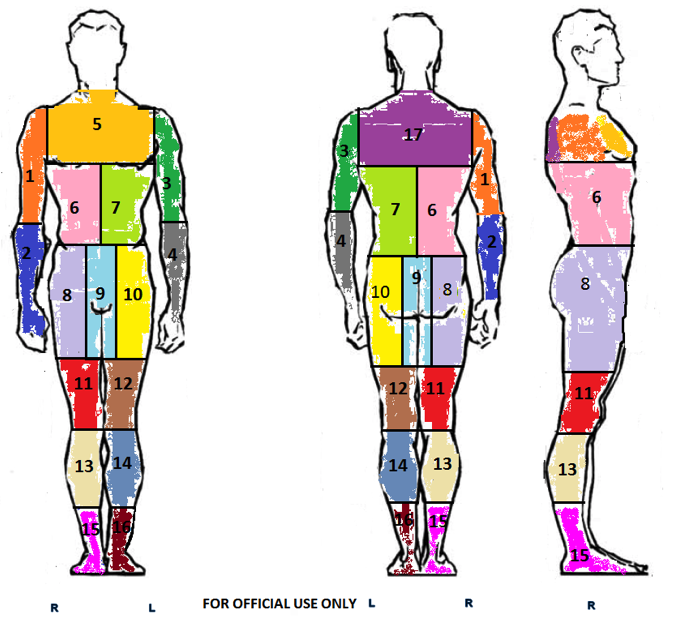
\includegraphics[width=.5\textwidth]{../Pic/body_zones}
\caption{17 regions of a typical human being defined by TSA}
\label{fig:17Region}
\end{figure}

TSA released a set of data containing thousands of packages of images screened by Millimeter Wave Unit, within each of which there are 16 frames of monochrome images shoot from different perspectives around a single passenger. Each perspective has a rotation of 22.5 degrees to the previous one, and each image is of size $512\times660$. Moreover, a typical human being in screening process should contain 17 regions as shown in figure~\ref{fig:17Region} with its detailed definitions given in table~\ref{tbl:17Region}. Any potentially applicable algorithms should be able to identify any threatening items concerning these regions. However, the problem comes from the provided data: first, there is no or little features and noise is relatively significant; the training is not easy since those labeled data are not well-labeled. Almost every person has half of his regions' labels missing. Plus, the positive labels are of a small amount. Out of 1k people and 10k labels, there are only about 1k positive labels; finally, the computation resource is limited concerning the size of the dataset. Low-resolution images can take 10M per person.

We experimented the sparse representation approach with PCA on cropped regional images, but the result is not ideal. Since there are several regions are occluded from particular perspectives. Inspired by the inherent multi-view structure of the provided dataset, we built a Multi-view convolutional network with attention model to deal with the regional structure of TSA defined human being.

\begin{table*}[!htb]
\centering
\resizebox{\textwidth}{!}{%
\begin{tabular}{|l|l|l|}
\hline
\multicolumn{1}{|c|}{\textbf{Region}} & \textbf{Region Name} & \textbf{Region Location Description} \\ \hline
1 & Right Bicep & Top of the right shoulder to just above the elbow \\ \hline
2 & Right Forearm & Elbow to the fingertips \\ \hline
3 & Left Bicep & Top of the right shoulder to just above the elbow \\ \hline
4 & Left Forearm & Elbow to the fingertips \\ \hline
5 & Upper Chest & Front of the body \\ \hline
6 & Right Rib Cage and Abs & From the bottom of the pectoral muscle to the top of the waistline, center of the back, rib cage on the right side \\ \hline
7 & Left Rib Cage and Ab & From the bottom of the pectoral muscle to the top of the waistline, center of the back, rib cage on the left side \\ \hline
8 & Upper Right Hip / Thigh & Waistline to the half of person's thigh and extend to back including half of the right buttocks(pocket region) \\ \hline
9 & Groin(Sensitive Area) & Below the central part of the waist, includes part of the both right and left inner and upper thigh \\ \hline
10 & Upper Left Hip / Thigh & Waistline to the half of person's thigh and extend to back including half of the right buttocks(pocket region) \\ \hline
11 & Lower Right Thigh & Half of the lower right thigh - including the knee \\ \hline
12 & Lower Left Thigh & Half of the lower left thigh - including the knee \\ \hline
13 & Right Calf & Below the knee to the lower leg \\ \hline
14 & Left Calf & Below the knee to the lower leg \\ \hline
15 & Right Ankle Bone & Starts at the end of the calf muscle and includes the foot \\ \hline
16 & left Ankle Bone & Starts at the end of the calf muscle and includes the foot \\ \hline
17 & Upper Back & Upper half of the back(ends at the same point where the pectoral region stops) \\ \hline
\end{tabular}%
}
\caption{17 Regions Defined by TSA in Human Screening}
\label{tbl:17Region}
\end{table*}

\begin{figure*}[!t]
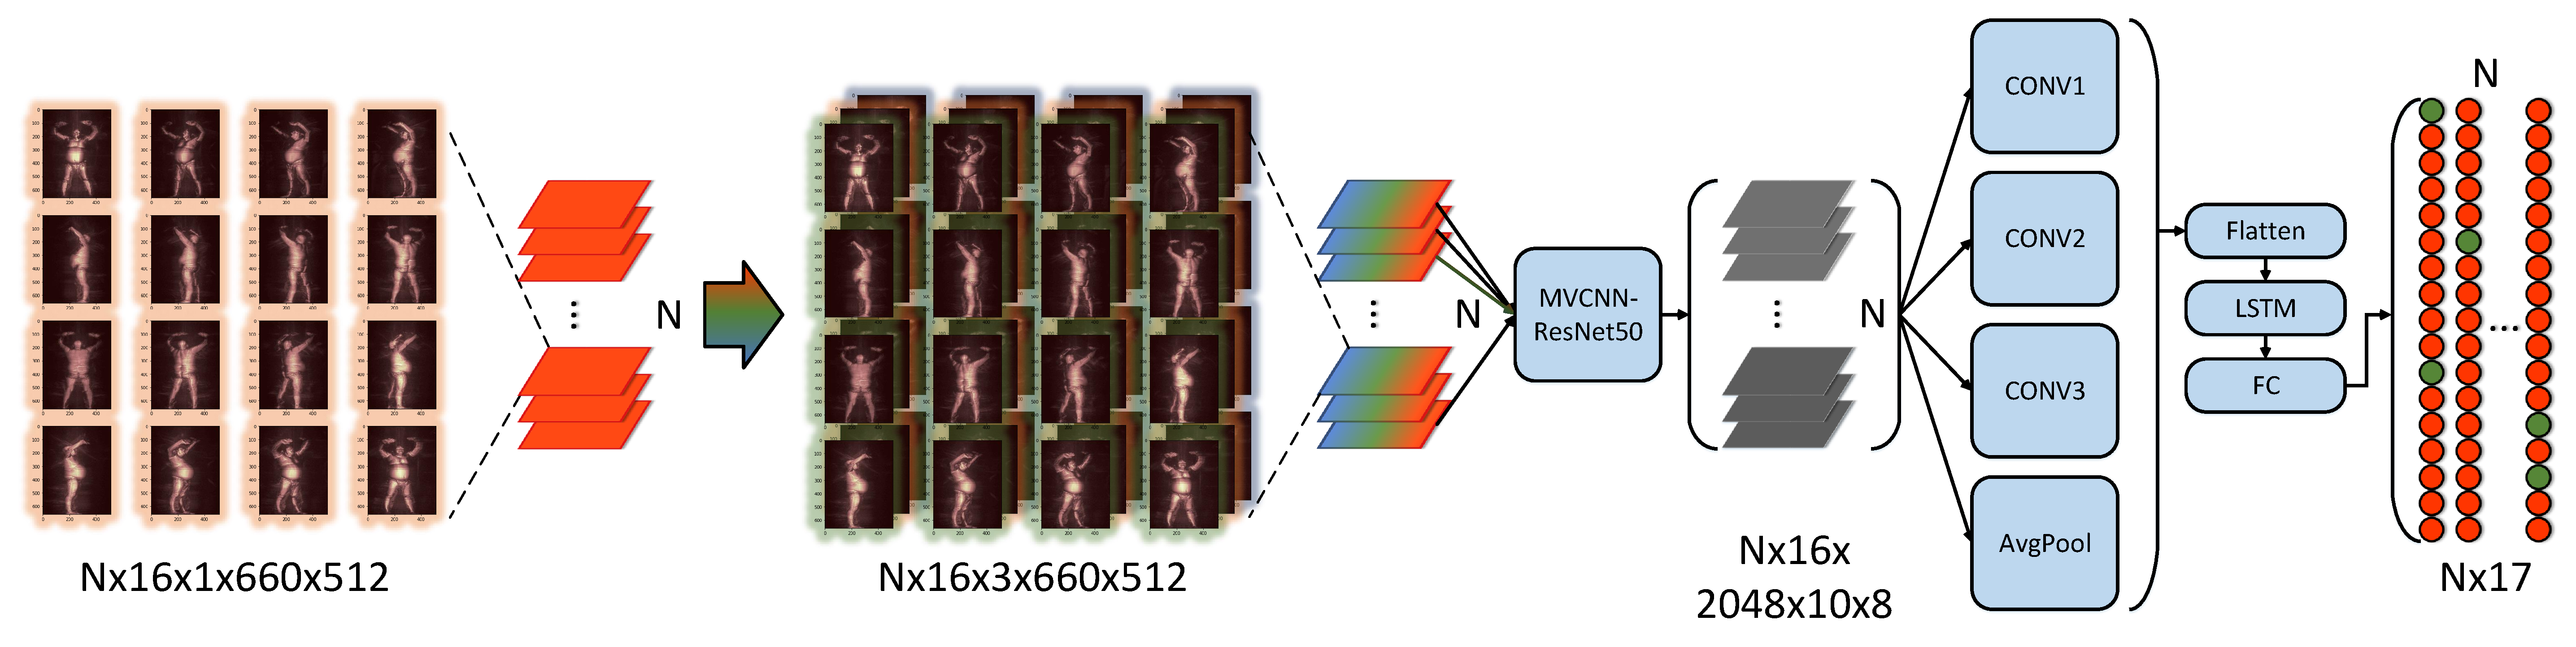
\includegraphics[width=\textwidth]{../Pic/Network.pdf}
\caption{Pipeline}
\label{network}
\end{figure*}

\section{Related Work}
Not much of work has been conducted on such topic. However, much research has been done regarding 3D object recognition. Although these are two different tasks, which have something in common.

We dived into these topics and realized that some of the work is using shape descriptors, and many of them, like Wu et al. \cite{wu20153d} are using voxel-based representation. However, voxel representation is not the privilege we have here, and even if we have that it would not help us in determining where is the dangerous object.
Not many researchers considered multi-view image before. Even though 3D structures like voxel-based representation present information that 2D images cannot, but the result from Multi-view CNN\cite{su15mvcnn}\cite{qi2016volumetric} has shown that a series of images can preserve enough information for recognition.

Another finding is that many researchers have been dedicated to improving training process. Of all of them, SGDR got our attention. It reported 3.14\% and 16.21\% error on CIFAR-10 and CIFAR-100. What's more important, it freed us from tuning an appropriate learning rate but a somewhat close one is good enough, let alone it can escape from local minimal to some extent.


\section{Our Approach}
Figure~\ref{network} presents our pipeline. The core of our algorithm is the MVCNN~\cite{su15mvcnn} with LSTM attention model. In MVCNN part we used a pre-trained ResNet50\cite{he2016deep} network for feature extraction. Then we will apply three different convolution layers and an avgpool, this is for extracting features from different scales. Their output is concatenated and flattened as a sequence, which is later fed to LSTM for quality refinement. The final layer is a fully-connected with output labels on 17 regions per individual image package.

We will show the dimension of the data after each section. Some Notations: $N$ stands for humans in a batch. $C$, $H$, $W$ stands for channels, height and width.

\subsection{MVCNN with Multi-colored Image}
The core of our network model is the multi-view CNN, a ResNet50 model which needs 3-channel images as input.
The grayscale image we got cannot be put into a 3-channel model directly. We duplicated the original image into three channels in all the testing below.
Thus the data sent to MVCNN has size $N\times16\times 3\times 660 \times 512$.

Each MVCNN will report 2048 channels of information with size $N \times 16 \times 2046 \times 10 \times 8$.
We have considered using the mean and variance of all humans of one pose as the other two channel, putting the original monochrome image as the red-channel. This alternative should be providing more insight than the naive duplication. This is still under testing.
\begin{figure}[!tp]
	\centering
	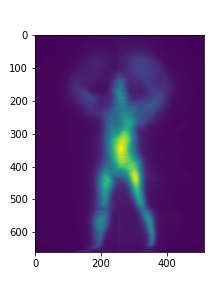
\includegraphics[width=.2\textwidth]{../Pic/mean_perspective_1}
	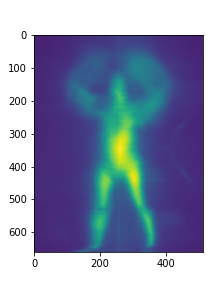
\includegraphics[width=.2\textwidth]{../Pic/std_perspective_1}
	\caption{Mean and Std of one pose.}
\end{figure}

\subsection{Convolution attention}
Our task is more difficult since we are not interested in the object, which already known as a human posed in certain ways. Rather, we are curious about the unnatural items hidden on the object which may or may not be visible and is significantly smaller than human. To accomplish this, we force an attention on it, which are three convolution layers of size $1\times1$, $3\times3$ and $5\times5$ to force the attention of different scale. 3 convolution should output data with size $N\times16\times512\times 10\times8$, $N\times16\times256\times5\times4$, $N\times16\times128\times4\times3$.

An average pool is also applied to take averages of the $10\times8$ image and thus provide average information which is missed because we did not fill the channels with mean and standard deviation. This layer will output size $N\times 16\times 2048$.

Another good thing about such practice: it reduced much of memory space.

\subsection{LSTM}
LSTM is good at sequential information. So we pressed the four layers above into a sequence of data with size $N\times(2048+512*10*8+256*5*4+128*4*3)$. After LSTM a weight will be calculated with softmax, and it will be applied to fully connected afterward.

\subsection{SGDR}
The basic idea of SGDR~\cite{SGDR} is to restart the learning rate after some time. Learning rate is controlled by a cosine function whose cycle increases each time one cycle concludes. It is reported that the error on CIFAR-10 and CIFAR-100 were 3.14\% and 16.21\% respectively.
\par We used the following formula to update our learning rate. The parameters are tuned as in \cite{SGDR}
$$ \eta_t = \eta_{min}^i + \frac{1}{2}(\eta_{max}^i-\eta_{min}^i)(1 + \cos(\frac{T_{curr}}{T_i}\pi))$$
$$ T_{i} = T_{i-1} * T_{mult} $$
We set $T_0$, $T_{mult}$ being 100 and 2 respectively. Others the same with the CosineAnnealingLR defined in pytorch


\section{Experiment}
To predict a True/False problem we choose to output a vector of dimension $17 \times 1$ with 17 probabilities.
We used Binary Cross Entropy to determine our error. However, it's still difficult to calculate errors when the labeled vector can be broken with only half of them being true.(Others are unlabeled and we decided them should be 0).
Below is a table and a Image we will use to show the training results of different network.
\par In practice we used lowest resolution(660*512), and a small batch size of 2, considering how much memory our model may take up.
\begin{figure}[!tp]
	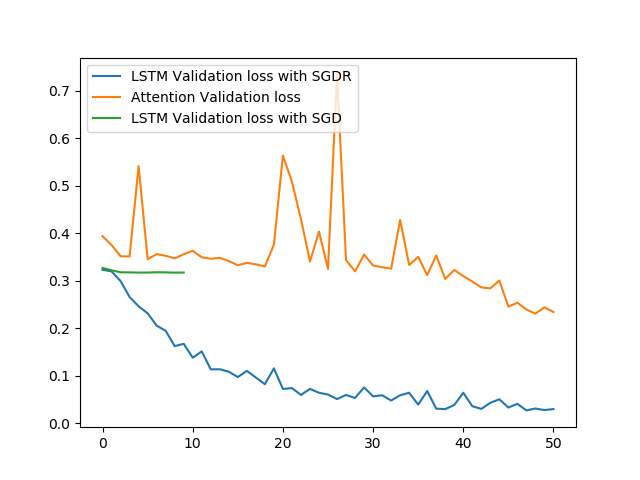
\includegraphics[width=.5\textwidth]{../Pic/3models}
	\caption{3 Main experiments we have done and their Validation loss}
\end{figure}
\par
It can be seen that without LSTM, MVCNN and attention together can't be used to train a good model, for similar information's correlation is ignored. But with the help of LSTM the loss can drop quickly. But it is worth mentioning even 50 epochs took almost 20 hours to train.
\par
Another indication is that simply SGD with decaying learning rate did poorly in terms of training. For 10 epochs there is almost no loss change. Thus we stopped the experiment, considering it would be meaningless to wait for it to drop to an acceptable level.(Likely it will take longer than 100 hours and we are short in GPU resource.)

\section{Discussion and other thinkings}
Since the provided data is monochrome and all of them are registered, we naturally came up with the idea of sparse representation. We experiment this idea on regional cropped images.

\subsection{Image Crop}
We have considered the possibility of taking 16 images with size of 660*512 images as input and a vector of size 17*1 describing the possibility of presence of dangerous objects. However, considering there isn't much positive outcomes, we decided to crop the images and for each zone, only see certain sector of the image.


The image is cropped into 16 sectors; each sector has size 250*250 pixels. The table listed the upper left corner of each sector:
\begin{table}[!htb]
    \centering
    \caption{My caption}
    \label{my-label}
    \begin{tabular}{ccc}
        \hline
        Region \# & x   & y   \\ \hline
        1         & 50  & 50  \\ \hline
        2         & 0   & 0   \\ \hline
        3         & 50  & 250 \\ \hline
        4         & 250 & 0   \\ \hline
        5         & 150 & 150 \\ \hline
        6         & 200 & 100 \\ \hline
        7         & 200 & 150 \\ \hline
        8         & 250 & 50  \\ \hline
        9         & 250 & 150 \\ \hline
        10        & 300 & 200 \\ \hline
        11        & 400 & 100 \\ \hline
        12        & 350 & 200 \\ \hline
        13        & 410 & 0   \\ \hline
        14        & 410 & 200 \\ \hline
        15        & 410 & 0   \\ \hline
        16        & 410 & 200 \\ \hline
    \end{tabular}
    \caption{Region distribution.}
\end{table}
\subsection{Zone assignment}
Now that we have already cropped each image, we will assign each region to its zones. This makes recognition on each zone easier. Now that no zone can be shown in all 16 images, we will represent it by a None in python.

We have done the pre-calculation to assign sectors based on the index of the image. For example, threat zone 1(Right Bicep) can be seen in sector 1 in image 0, 1, 2, 13, 14, 15; in sector 3 in image 6 to 10.

\subsection{Upsample}
For the data set given, for now, there are 1871 positive outcomes over 19500 samples, distributed all over 17 zones. This made our work harder because deep learning algorithms will be looking for more positive outcomes to learn.

We are upsampling the positive outcomes by duplicate positive outcomes and mirror positive images. Thus we will have more than 5000 positive images. It is unclear whether this is enough.

We are up sampling the positive outcomes by duplicate positive outcomes and mirror positive images. Thus we will be having more than 5000 positive images. It's unclear whether this is enough.

\subsection{Acknowledgement}
\par We would like to thank Peng Ding for drafing the milestone and final report and plotting the structure of our network. His idea of PCA was really brilliant and helpful and he devoted much time researching on that.

\bibliographystyle{IEEEtran}
\bibliography{report}
\end{document}
